\chapter{Introduction}
\minitoc

Between the SaX GUI and the SaX engine an interface exists to
transport the information from the GUI into the engine which
is then able to create or modify the X11 configuration. This
interface is called \textbf{ISaX}. A complete explanation about
how SaX2 is structured can be found within the documentation
at \textit{/usr/share/doc/packages/sax2}. 
The ISaX interface is the basis for the C++ library explained here.
The library is based on the following major topics:

\begin{enumerate}
\item \textbf{\underline{Init:}}\\
      Provide session cache
\item \textbf{\underline{Import:}}\\
      Provide classes to obtain all necessary information
\item \textbf{\underline{Manipulate:}}\\
      Provide classes to manipulate imported data
\item \textbf{\underline{Export:}}\\
      Provide classes to create or modify the X11-Configuration
\end{enumerate}

The programmer starts with an init() sequence to be able to
access the automatically generated configuration suggestion which is
based on the hardware detection. After this it is possible to
import,manipulate and export information.

\section{Rough diagram of SaX2 procedures}
To give an introduction about how the ISaX interface is working
as part of SaX2 the following rough overview will show the basics
of the SaX2 engine.

\newpage

\begin{figure}[h]
\caption{SaX2 Flow diagram}
\vspace*{0.2cm}
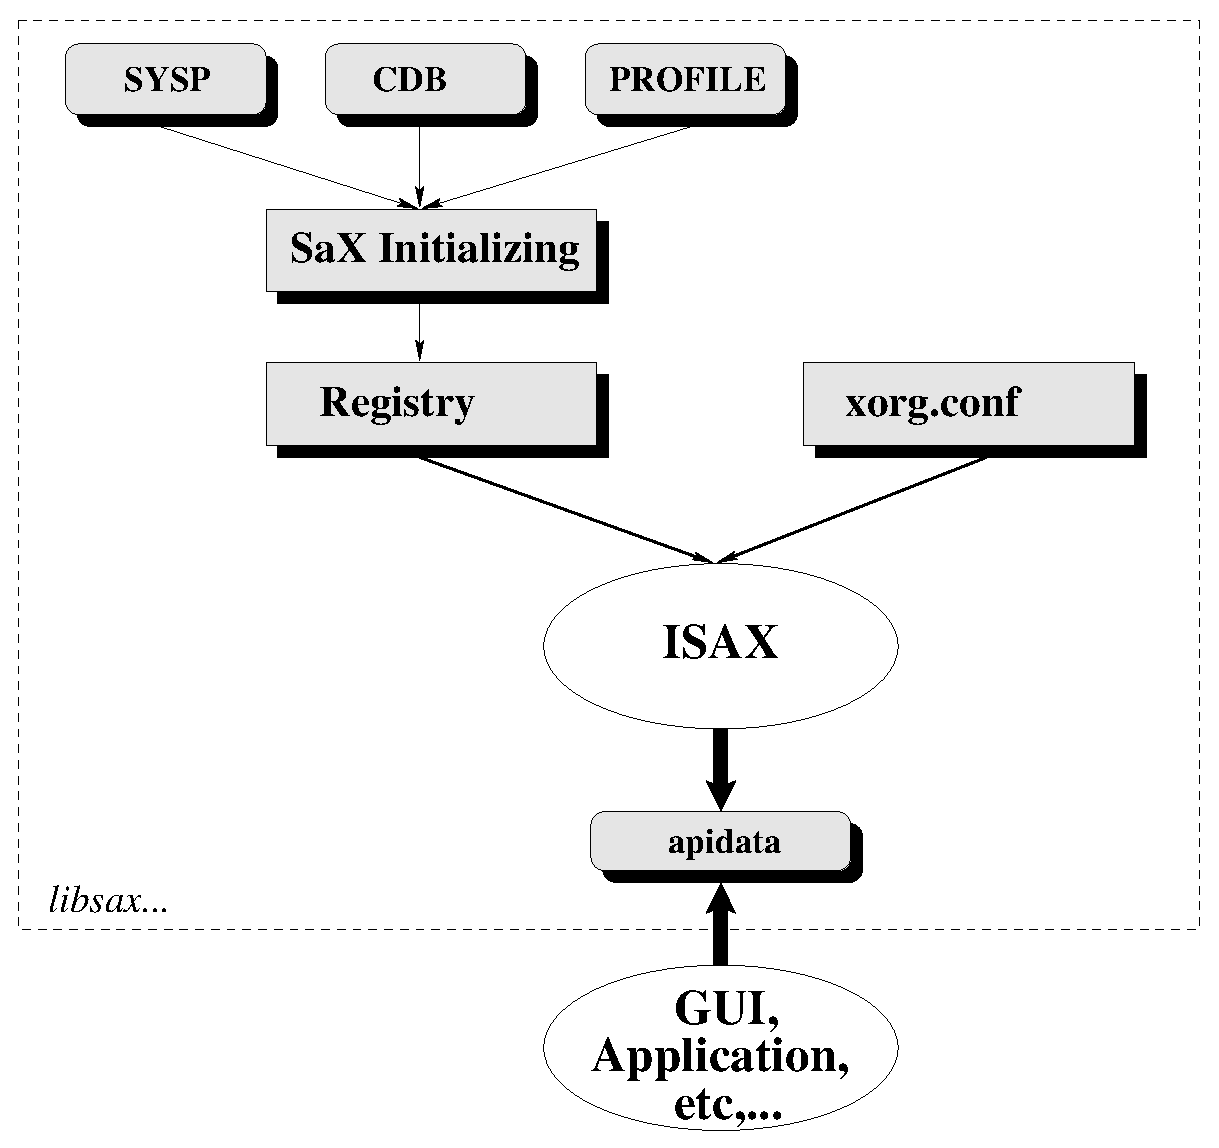
\includegraphics[scale=0.5]{pictures/sax.eps}
\end{figure}

\section{SaX Import Classes}
%The programmer starts with an init() sequence to be able to
%access the automatically generated configuration suggestion which is
%based on the hardware detection. After this it is possible to
%import a set of information. Following import methods are available:
\begin{itemize}
\item \textbf{\underline{ISAX}}\\
      The data of the currently used X11 configuration or the automatically
      generated configuration suggestion can be obtained by using the ISaX
      interface respectively by using the \textbf{isax} command. The
      information is stored into \textbf{SaXImport} objects.
\item \textbf{\underline{SYSP}}\\
      Information near to the hardware like PCI IDs, BusID, etc... can be
      obtained by using the Sysp interface respectively by using the
      \textbf{sysp} command. The information is stored into
      \textbf{SaXImportSysp} objects
\item \textbf{\underline{CDB}}\\
      Manually maintained data refering stuff like Mice, Tablets,
      Graphics Cards, Monitors, etc... can be obtained from the exported
      files of the CDB (Component Data-Base). The information is stored
      into \textbf{SaXImportCDB} objects
\item \textbf{\underline{PROFILE}}\\
      Profile information for a specific card can be obtained using a
      special ISaX interface script called \textit{createPRO.pl}. The
      information given here is stored into a \textbf{SaXImportProfile}
      object.
\end{itemize}

\newpage

\section{SaX Manipulation Classes}
Once the needed data has been imported the programmer can start to
manipulate it. The information from the SYSP, CDB and PROFILE methods
are helpful but only the data concerning the ISAX import are used for
the later export respectively the later configuration file. If the
programmer is familiar with the ISaX interface there would be no need
to provide further manipulation classes but to make it comfortable
the library should provide SaXManipulation... classes to be able to
do the common configuration tasks easily. At this point we need to
define what the common configuration tasks are. Currently the following
manipulation classes are specified:

\begin{itemize}
\item Baseclass: \textbf{\underline{SaXManipulateCard}}\\
      Handle hardware related configuration settings including
      stuff like graphics drivers options etc...
\item Baseclass: \textbf{\underline{SaXManipulateDesktop}}\\
      Handle desktop related configuration settings including
      stuff like resolution colordepth etc...
\item Baseclass: \textbf{\underline{SaXManipulateDevices}}\\
      Handle device creation including stuff like creating or
      deleting a desktop adding input devices etc...
\item Baseclass: \textbf{\underline{SaXManipulateExtensions}}\\
      Subclass:\hspace*{0.2cm} \textit{SaXManipulateVNC}\\
      Handle X-Server extensions for example VNC
\item Baseclass: \textbf{\underline{SaXManipulateKeyboard}}\\
      Handle keyboard configuration settings
\item Baseclass: \textbf{\underline{SaXManipulateLayout}}\\
      Handle layout configuration settings of multihead
      environments
\item Baseclass: \textbf{\underline{SaXManipulatePath}}\\
      Handle fontpath serverflags and server modules configuration settings
\item Baseclass: \textbf{\underline{SaXManipulatePointers}}\\
      Subclass:\hspace*{0.2cm} \textit{SaXManipulateMice,SaXManipulateTablets,SaXManipulateTouchscreens}\\
      Handle pointer devices including stuff like mice tablets or
      touchscreen configuration settings
\end{itemize}
 
After all manipulations to all \textbf{SaXImport} objects have been done
the programmer needs to add the affected SaXImport objects to a
\textbf{SaXConfig} object which handles the export. 

\section{SaX Export Classes}
the library provides a \textbf{SaXExport} and a \textbf{SaXConfig} class
whereas the SaXConfig class is able to include multiple SaXImport objects.
The SaXConfig object will create a corresponding SaXExport object for each
SaXImport object bound to the SaXConfig object. With this list of SaXExport
objects it is possible to create a new - or modify an existing X11
configuration.

\section{libsax classes and inheritance}
\begin{figure}[h]
\caption{libsax: object reference}
\vspace*{0.1cm}
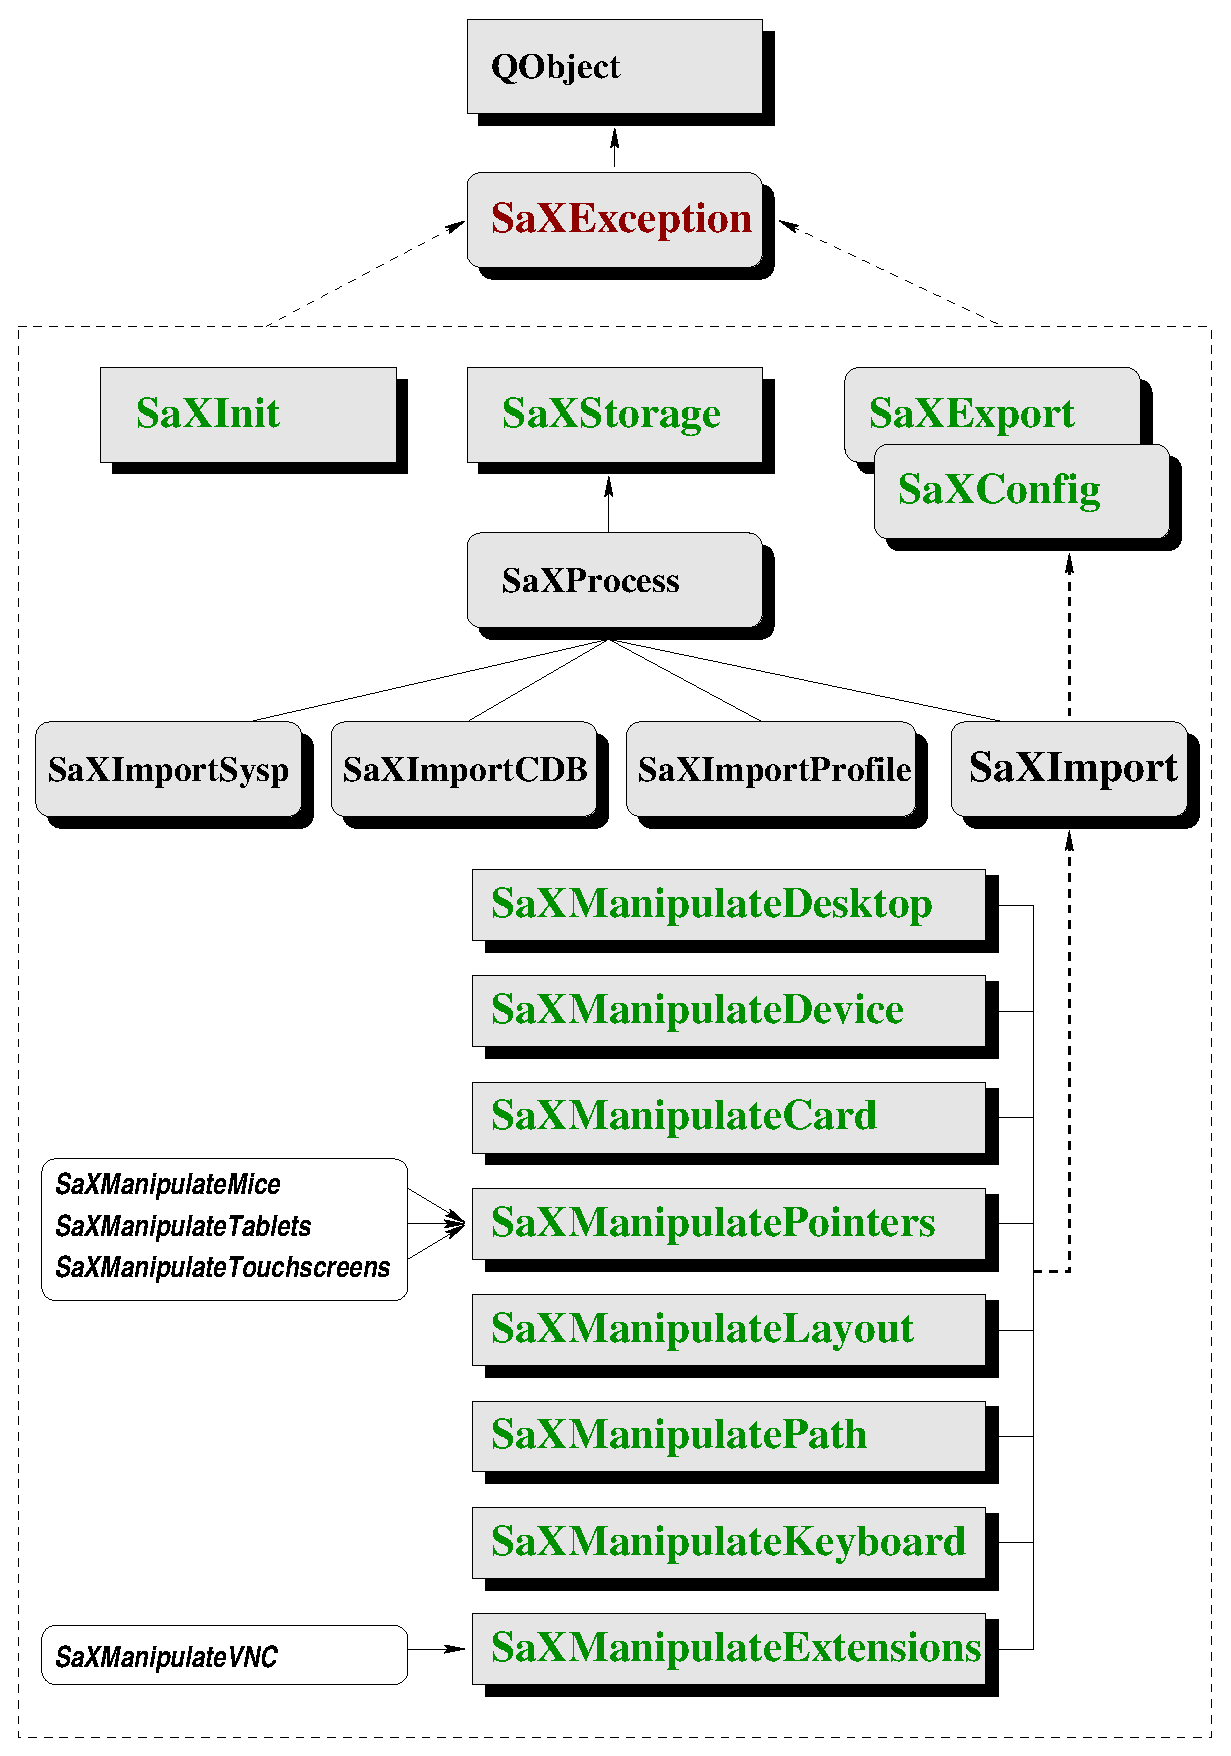
\includegraphics[scale=0.5]{pictures/tree.eps}
\end{figure}
